\documentclass{ximera}

\newcommand{\RR}{\mathbb R}
\renewcommand{\d}{\,d}
\newcommand{\dd}[2][]{\frac{d #1}{d #2}}
\renewcommand{\l}{\ell}
\newcommand{\ddx}{\frac{d}{dx}}
\newcommand{\dfn}{\textbf}
\newcommand{\eval}[1]{\bigg[ #1 \bigg]}


\outcome{Compute $\frac{dy}{dx}$ from the polar representation of a curve.}
\outcome{Determine where $\frac{dy}{dx}$ of a polar curve is zero or undefined.}
\outcome{Find the equation of a tangent line to the polar representation of a curve.}

\title[Dig-In:]{Derivatives of polar functions}

\begin{document}
\begin{abstract}
  We differentiate polar functions.
\end{abstract}
\maketitle

The previous section discussed a special class of parametric functions
called polar functions.  We know that
\begin{align*}
  \d x &= x'(t) \d t\\
  \d y &= y'(t) \d t,
\end{align*}
and so we can compute the derivative of $y$ with respect to $x$ using
differentials:
\[
\frac{\d y}{\d x} = \frac{y'(t) \d t}{x'(t) \d t} = \frac{y'(t)}{x'(t)}
\]
provided that $x'(t) \ne 0$.  With polar functions we have
\begin{align*}
  x(\theta) &= r(\theta) \cdot \cos(\theta) \\
  y(\theta) &= r(\theta) \cdot \sin(\theta),
\end{align*}
so
\begin{align*}
\dd[y]{x} &= \frac{y'(\theta)}{x'(\theta)} \\
&= \frac{r'(\theta) \sin(\theta)+r(\theta) \cos(\theta)}{r'(\theta)\cos(\theta)-r(\theta)\sin(\theta)}
\end{align*}
provided that $x'(\theta)\ne 0$.

\begin{example}
  Consider the lima\c{c}on $r(\theta) =1+2\sin(\theta)$ on the interval $[0,2\pi]$:
  \begin{image}
     \begin{tikzpicture}
          \begin{polaraxis}[
              xtick={0,45,...,360},
              xticklabels={$0$,$\frac{\pi}{4}$,$\frac{\pi}{2}$,$\frac{3\pi}{4}$,$\pi$,$\frac{5\pi}{4}$,$\frac{3\pi}{2}$,$\frac{7\pi}{4}$,$2\pi$},
            ]
            \addplot+[very thick, mark=none,penColor,domain=0:360,samples=100,smooth] {1+2*sin(x)};
          \end{polaraxis}
     \end{tikzpicture}
  \end{image}
  Find the equation of the tangent line to the curve at $\theta=\pi/4$.
  \begin{explanation}
    We start by computing the derivative in rectangular coordinates. Recall that
    \begin{align*}
      x(\theta) &= \left(1+2\sin(\theta)\right)\cdot \cos(\theta) = \cos(\theta)+2\sin(\theta)\cos(\theta)\\
      y(\theta) &= \left(1+2\sin(\theta)\right)\cdot \sin(\theta) = \sin(\theta)+2\sin^2(\theta)
    \end{align*}
    Consequently,
    \begin{align*}
      x'(\theta) &= \answer[given]{-\sin(\theta) + 2\cos^2(\theta)-2\sin^2(\theta)} \\
      y'(\theta) &= \answer[given]{\cos(\theta) + 4\sin(\theta)\cos(\theta)}
    \end{align*}
    and therefore
    \[
    \dd[y]{x} = \answer[given]{\frac{\cos(\theta) + 4\sin(\theta)\cos(\theta)}{-\sin(\theta) + 2\cos^2(\theta)-2\sin^2(\theta)}}.
    \]
    When $\theta=\pi/4$,
    \begin{align*}
      x(\theta) &= \answer[given]{1+\sqrt{2}/2}\\
      y(\theta) &=\answer[given]{1+\sqrt{2}/2}\\
    \dd[y]{x} &=\answer[given]{-2\sqrt{2}-1}
    \end{align*}
     Thus the equation of the line (in \wordChoice{\choice{polar}\choice[correct]{rectangular}} coordinates) tangent to the lima\c{c}on at $\theta=\pi/4$ is
     \[
     y=(-2\sqrt{2}-1)\big(x-(1+\sqrt{2}/2)\big)+1+\sqrt{2}/2 \approx  -3.83 x+8.24.
     \]
    \begin{prompt}
      \[
      \graph{r=1+2\sin(\theta), y=(-2\sqrt{2}-1)(x-(1+\sqrt{2}/2))+1+\sqrt{2}/2}
      \]
    \end{prompt}
  \end{explanation}
\end{example}





\begin{example}
  Consider the lima\c{c}on given by $r(\theta) =1+2\sin(\theta)$ on the
  interval $[0,2\pi]$.  Find Cartesian coordinates for the points
  where the tangent line to this lima\c{c}on is horizontal.
\begin{explanation}
  To find these points where the tangent lines is horizontal, we seek
  points where $\dd[y]{x} = \answer[given]{0}$.  From earlier, we discovered
  \[
  \dd[y]{x} =\frac{\cos(\theta) + 4\sin(\theta)\cos(\theta)}{-\sin(\theta) + 2\cos^2(\theta)-2\sin^2(\theta)}
  \]
  so now we must find where the numerator is $0$. Since the numerator is equal to
  \[
  \cos(\theta)(1+ 4\sin(\theta))
  \]
  and since a product is zero when \wordChoice{\choice{both}\choice[correct]{either}} of the terms is zero,
  the numerator is zero when 
  \begin{itemize}
  \item $\cos(\theta)=0$ or
  \item $1+4\sin(\theta)=0$.
  \end{itemize}

  Let's examine the case of $\cos(\theta) = 0$ first, and restrict to the situation where $\theta$ is between $0$ and $2\pi$.
  If $\theta$ is in the interval $[0,\pi]$, then $\cos(\theta)=0$ when $\theta=\answer[given]{\pi/2}$.
  If $\theta$ is in the interval $[\pi,2\pi]$, then $\cos(\theta)=0$ when $\theta=\answer[given]{3\pi/2}$.

  The corresponding points in rectangular coordinates are
  \begin{align*}
    x(\pi/2) &= \left(1+2\sin(\pi/2)\right)\cdot\cos(\pi/2)\\
    &= 0,\\
    y(\pi/2) &= \left(1+2\sin(\pi/2)\right)\cdot\sin(\pi/2)\\
    &= 3,
  \end{align*}
  meaning $(x,y) = (0,3)$, and
  \begin{align*}
    x(3\pi/2) &= \left(1+2\sin(3\pi/2)\right)\cdot\cos(3\pi/2)\\
    &= 0,\\
    y(3\pi/2) &= \left(1+2\sin(3\pi/2)\right)\cdot\sin(3\pi/2)\\
    &= 1,
  \end{align*}
  meaning $(x,y) = (0,1)$.

  But the numerator was the product of $\cos(\theta)$ and another term, namely $1+4\sin(\theta)$  So the numerator is also zero when
  \begin{align*}
    1+4\sin(\theta)&=0\\ 4\sin(\theta)&=-1\\ \sin(\theta)&=\frac{-1}{4}.
  \end{align*}
  At this point we have a choice to make: We can either apply the
  arcsin function and solve for $\theta$, or we can work with
  $\sin(\theta)$ directly. Perhaps the easier route is to work with
  $\sin(\theta)$ directly. To explore $\sin(\theta)$, we may choose an
  algebraic method employing the Pythagorean identity, or a geometric
  method looking at the unit circle with the Pythagorean
  theorem. Let's take the geometric route to compute $\cos(\theta)$.
  \begin{image}
    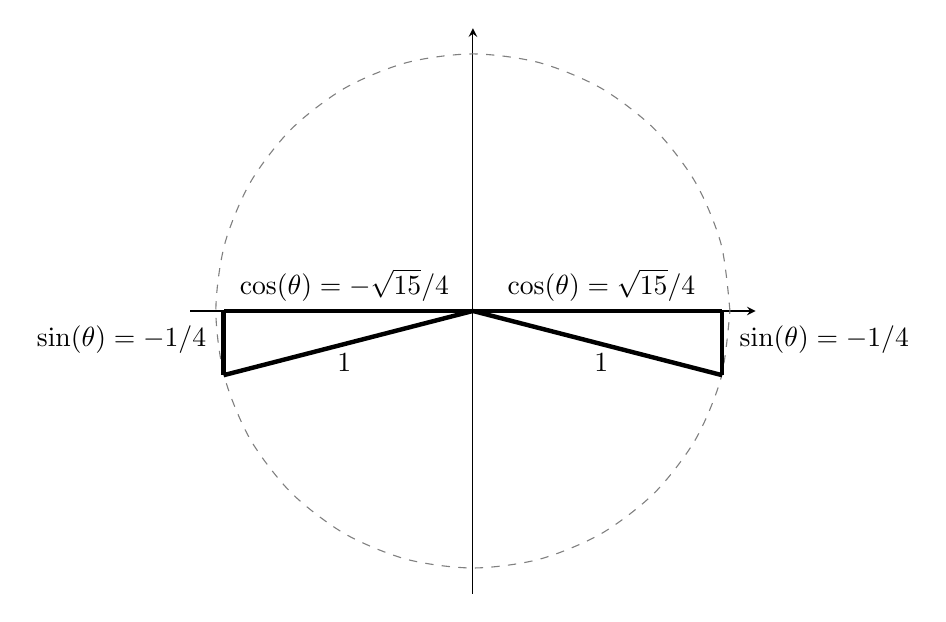
\begin{tikzpicture}
      \begin{axis}[
          xmin=-1.1,xmax=1.1,ymin=-1.1,ymax=1.1,
          axis lines=center,
          width=4in,
          ticks=none,
          clip=false,
          unit vector ratio*=1 1 1,
          %xlabel=$x$, ylabel=$y$,
          every axis y label/.style={at=(current axis.above origin),anchor=south},
          every axis x label/.style={at=(current axis.right of origin),anchor=west},
        ]        
        \addplot [black!50!white, dashed, smooth, domain=(0:360)] ({cos(x)},{sin(x)}); %% unit circle
        
        \addplot [ultra thick] plot coordinates {(0,0) (.97,-.25)}; 
        \addplot [ultra thick] plot coordinates {(.97,0) (.97,-.25)}; 
        \addplot [ultra thick] plot coordinates {(0,0) (.97,0)};

        \addplot [ultra thick] plot coordinates {(0,0) (-.97,-.25)}; 
        \addplot [ultra thick] plot coordinates {(-.97,0) (-.97,-.25)}; 
        \addplot [ultra thick] plot coordinates {(0,0) (-.97,0)}; 

        \node at (axis cs:-.5,-.2) {$1$};
        \node at (axis cs:.5,-.2) {$1$};
        \node[anchor=west] at (axis cs:1,-.11) {$\sin(\theta) = -1/4$};
        \node[anchor=east] at (axis cs:-1,-.11) {$\sin(\theta) = -1/4$};
        \node[anchor=south] at (axis cs:-.5,0) {$\cos(\theta) = -\sqrt{15}/4$};
        \node[anchor=south] at (axis cs:.5,0) {$\cos(\theta) = \sqrt{15}/4$};
        
      \end{axis}
    \end{tikzpicture}
  \end{image}
  Hence the derivative \wordChoice{\choice[correct]{is zero}\choice{is one}\choice{is undefined}} at
  \begin{align*}
    x(\theta) &= \left(1+2\sin(\theta)\right)\cdot\cos(\theta)\\
    &= \left(1+2(-1/4)\right)\cdot \sqrt{15}/4\\
    &= \sqrt{15}/8,\\
    y(\theta) &= \left(1+2\sin(\theta)\right)\cdot\sin(\theta)\\
    &= \left(1+2(-1/4)\right)\cdot (-1/4)\\
    &= -1/8,
  \end{align*}
  meaning $(x,y) = (\sqrt{15}/8, -1/8)$, and
   \begin{align*}
    x(\theta) &= \left(1+2\sin(\theta)\right)\cdot\cos(\theta)\\
    &= \left(1+2(-1/4)\right)\cdot (-\sqrt{15}/4)\\
    &= -\sqrt{15}/8,\\
    y(\theta) &= \left(1+2\sin(\theta)\right)\cdot\sin(\theta)\\
    &= \left(1+2(-1/4)\right)\cdot (-1/4)\\
    &= -1/8,
  \end{align*}
   meaning $(x,y) = (-\sqrt{15}/8, -1/8)$.

   In summary, the graph of $r(\theta) = 1+2\sin(\theta)$ on the interval $[0,2\pi]$
   has horizontal tangent lines at the points
   \begin{itemize}
   \item $(x,y) = (0,\answer[given]{3})$,
   \item $(x,y) = (0,1)$,
   \item $(x,y) = (\sqrt{15}/8, -1/8)$, and 
   \item $(x,y) = (-\sqrt{15}/8, -1/8)$.
   \end{itemize}
   \begin{prompt}
     You can confirm this by looking at the graph below:
     \[
     \graph{r=1+2\sin(\theta),y=3,y=1,y=-1/8}
     \]
   \end{prompt}
\end{explanation}
\end{example}


\begin{example}
  Again consider our friend the lima\c{c}on given by $r(\theta)
  =1+2\sin(\theta)$ on the interval $[0,2\pi]$.  Find Cartesian
  coordinates for the points where the tangent line to this lima\c{c}on
  is vertical.
  \begin{explanation}
    To find the vertical tangent lines, we seek points where the
    denominator of
    \[
    \dd[y]{x}=\frac{\cos(\theta) + 4\sin(\theta)\cos(\theta)}{-\sin(\theta) + 2\cos^2(\theta)-2\sin^2(\theta)}
    \]
    is equal to zero.  To start, we will convert $\cos^2(\theta)$ to
    $1-\answer[given]{\sin^2(\theta)}$, and express the denominator as a quadratic
    expression in $\sin(\theta)$:
  \begin{align*}
    -\sin(\theta) + 2\cos^2(\theta)-2\sin^2(\theta) & = -\sin(\theta) + 2(1-\sin^2(\theta))-2\sin^2(\theta) \\
    &= \answer[given]{-4} \sin^2(\theta) + \answer[given]{-1}\sin(\theta) + \answer[given]{2}.
  \end{align*}
  We then set this equal to zero and note that the equation is quadratic equation in the variable $\sin(\theta)$. The quadratic formula gives that 
  \begin{align*}
    \sin(\theta) &= \frac{-1\pm\sqrt{\answer[given]{33}}}{8}.
  \end{align*}
  Now we can find cosine using either geometrically via the unit circle or algebraically with the Pythagorean
  identity.  This time, let's take the more algebraic route with the Pythagorean identity. When $\sin(\theta) =\frac{-1+\sqrt{33}}{8}$, then
  \begin{align*}
    \cos^2(\theta) + \sin^2(\theta) &= 1\\
    \cos^2(\theta) + \left(\frac{-1+\sqrt{33}}{8}\right) &= 1.
  \end{align*}
  So
  \[
  \cos(\theta) = \pm \frac{\sqrt{(\answer[given]{15}+\sqrt{33})/2}}{4}
  \]
  and when $\sin(\theta) =\frac{-1-\sqrt{33}}{8}$,
  \begin{align*}
    \cos^2(\theta) + \sin^2(\theta) &= 1\\
    \cos^2(\theta) + \left(\frac{-1-\sqrt{33}}{8}\right) &= 1.
  \end{align*}
  So
  \[
  \cos(\theta) = \pm \frac{\sqrt{(\answer[given]{15}-\sqrt{33})/2}}{4}.
  \]
  So now we know that the graph of $r(\theta) =1+2\sin(\theta)$ on
  $[0,2\pi]$ has vertical tangent lines at the four points
   \begin{image}
      \begin{tikzpicture}
        \node at (0,0) {
          $\begin{aligned}
          (\cos(\theta),\sin(\theta)) = \left(\frac{\sqrt{(15+\sqrt{33})/2}}{4},\frac{-1+\sqrt{33}}{8}\right),\\
          (\cos(\theta),\sin(\theta)) = \left(\frac{-\sqrt{(15+\sqrt{33})/2}}{4},\frac{-1+\sqrt{33}}{8}\right),\\
          (\cos(\theta),\sin(\theta)) = \left(\frac{\sqrt{(15-\sqrt{33})/2}}{4},\frac{-1-\sqrt{33}}{8}\right), \\ 
          (\cos(\theta),\sin(\theta)) = \left(\frac{-\sqrt{(15-\sqrt{33})/2}}{4},\frac{-1-\sqrt{33}}{8}\right).
          \end{aligned}$
        };
      \end{tikzpicture}
   \end{image}
   Recalling that
   \begin{align*}
     x(\theta) &= \left(1+2\sin(\theta)\right)\cdot\cos(\theta)\\
     y(\theta) &= \left(1+2\sin(\theta)\right)\cdot\sin(\theta)
   \end{align*}
   we see that the graph of $r(\theta) =1+2\sin(\theta)$ on $[0,2\pi]$
   has vertical tangent lines at
    \begin{image}
      \begin{tikzpicture}
        \node at (0,0) {
          $\begin{aligned}
            (x,y) &= \left(\left(1+\frac{-1+\sqrt{33}}{4}\right)\frac{\sqrt{(15+\sqrt{33})/2}}{4},\left(1+\frac{-1+\sqrt{33}}{4}\right)\frac{-1+\sqrt{33}}{8}\right),\\
            (x,y) &= \left(\left(1+\frac{-1+\sqrt{33}}{4}\right)\frac{-\sqrt{(15+\sqrt{33})/2}}{4},\left(1+\frac{-1+\sqrt{33}}{4}\right)\frac{-1+\sqrt{33}}{8}\right),\\
            (x,y) &= \left(\left(1+\frac{-1-\sqrt{33}}{4}\right)\frac{\sqrt{(15-\sqrt{33})/2}}{4},\left(1+\frac{-1-\sqrt{33}}{4}\right)\frac{-1-\sqrt{33}}{8}\right),\\
            (x,y) &= \left(\left(1+\frac{-1-\sqrt{33}}{4}\right)\frac{-\sqrt{(15-\sqrt{33})/2}}{4},\left(1+\frac{-1-\sqrt{33}}{4}\right)\frac{-1-\sqrt{33}}{8}\right).
          \end{aligned}$
        };
      \end{tikzpicture}
    \end{image}
   
   \begin{prompt}
     You can confirm this visually by looking at the graph below:
     \[
     \graph{r=1+2\sin(\theta),
       x=\left(1+\frac{-1+\sqrt{33}}{4}\right)\frac{\sqrt{(15+\sqrt{33})/2}}{4},
       x=\left(1+\frac{-1+\sqrt{33}}{4}\right)\frac{-\sqrt{(15+\sqrt{33})/2}}{4},
       x=\left(1+\frac{-1-\sqrt{33}}{4}\right)\frac{\sqrt{(15-\sqrt{33})/2}}{4},
       x=\left(1+\frac{-1-\sqrt{33}}{4}\right)\frac{-\sqrt{(15-\sqrt{33})/2}}{4}}
     \]
   \end{prompt}
  \end{explanation}
\end{example}

When the graph of the polar function $r(\theta)$ intersects the origin
(sometimes called the ``pole''), then $r(\alpha)=0$ for some angle
$\alpha$.

\begin{question}
  When $r(\alpha) = 0$, what is the formula for $\dd[y]{x}$?
\begin{multipleChoice} 
  \choice{$\dd[y]{x}= \sin(\alpha)$.}
  \choice{$\dd[y]{x}= \cos(\alpha)$.}  
  \choice[correct]{$\dd[y]{x}= \tan(\alpha)$.}
\end{multipleChoice}
\end{question}
The answer to the question above leads us to an interesting point. It
tells us the slope of the tangent line at the pole.  When a polar
graph touches the pole at $\theta=\alpha$, the equation of the tangent
line in polar coordinates at the pole is $\theta=\alpha$.


\begin{example}
  Find the equations of the lines tangent to the graph of
  $r(\theta)=1+2\sin(\theta)$ at the pole.
  \begin{explanation}
    We need to know when $r(\theta)=0$.
    \begin{align*}
      1+2\sin(\theta) &= 0\\
      \sin(\theta) &= -1/2\\
      \theta &= \frac{7\pi}{6},\ \frac{\answer[given]{11}\pi}6.
    \end{align*}
    Thus the equations of the tangent lines, in \wordChoice{\choice[correct]{polar}\choice{rectangular}} coordinates, are
    \begin{align*}
      \theta &=7\pi/6 \theta \\
      \theta &= \answer[given]{11}\pi/6.
    \end{align*}
    In rectangular form, the tangent lines are $y=\tan(7\pi/6)x$ and
    $y=\answer[given]{\tan(11\pi/6)}x$.
    \begin{prompt}
     You can confirm this by looking at the graph below:
     \[
     \graph{r=1+2\sin(\theta),y=\tan(7\pi/6)x,y=\tan(11\pi/6)x}
     \]
   \end{prompt}
  \end{explanation}
\end{example}
\end{document}
















